\documentclass[12pt]{report}
\usepackage{epsfig}
\usepackage{upcebumath}  
\usepackage{UPnotations}
\usepackage{amssymb, graphicx, amsmath}
\usepackage{hyperref}
\usepackage{rotating}
\def\span{\mbox{\rm span}\,}
\usepackage{amsmath,latexsym}
\usepackage{amsbsy}
\usepackage{indentfirst}
\input graphtex

\newtheorem{thm}{Theorem}[section]
\newtheorem{lem}{Lemma}[section]
\newtheorem{thmcor}{Corollary}[thm]
\newtheorem{lemcor}{Corollary}[lem]
\newtheorem{defn}{Definition}[section]
\newtheorem{e.g.}{Example}[section]
\newtheorem{r.m.}{Remark}[section]
\newcommand{\proof}{\medskip \noindent\emph{Proof}:\ }
\newcommand{\qed}{$\Box$}
%\newcommand{\F}{\mathbb{F}}	

\begin{document}

\title{Molecular Topological Index of Monocyclic Graph $C_k(s,t)$} %do not capitalize all

\authorfirst{Krisell L.}
\authorlast{Abella}
%\authorext{Jr.} \authorexttrue %make this a comment if you do not have an extension name e.g. Jr., II, III, etc.

\degree{Bachelor of Science in Mathematics}
\thesistype{Undergraduate Thesis}
\thesisdocument{Thesis}

\defensedate{October 29, 2009} %indicate the month, day and year the research was defended
\submitmonth{November} %indicate the month the manuscript was submitted to the CS office
\submityear{2009} %indicate the year the manuscript was submitted to the Math Office


\adviser{John Benedict T. Ayawan}%main adviser
\reader{Precious Jane F. Lapura} %thesis panel

%%%%%%%%%%%%%%%%%%%%%%%%%%%%%%%%%%%%%%%%%%%%%%%%%%%%%%%
%% highlight \bothabsenttrue if the student has only one adviser and one reader
%% otherwise comment \bothabsenttrue and highlight \coadviser or \coreader which 
%% ever is applicable. In this case, the package assumes either you have 1 Adviser 
%% and 2 Readers, or 2 Advisers and 1 Reader. 
  
\bothabsenttrue

\coadviser{co-Adviser, Ph.D.} 
%\coadvisetrue  
% Make the \coadvisetrue as a comment if there is no adviser

%\coreader{Co-Reader's Name}  %leave this blank if there is a coadviser

%%%%%%%%%%%%%%%%%%%%%%%%%%%%%%%%%%%%%%%%%%%%%%%%%%%%%%%

\chairman{Jonnifer R. Sinogaya, Ph.D.} 

\abs{Type your abstract here.  Your abstract should have a minimum
of 150 words and a maximum of 300 words.}

\acknowledge{Type your acknowledgements here. It is customary to acknowledge special assistance from
extramural agencies. There is no obligation that assistance received from members of the dissertation or
thesis committee be acknowledged. \medskip

Acknowledgments should be couched in terms consistent with the
scholarly nature of the work. Your name and the date should not appear on this page.}

%\biodatatrue 
\beforepreface
\tableofcontents

\newpage

\acknowledgetrue
\acknowledgepage

\abstractpage
\listoftables
\listoffigures

\afterpreface

\chapter{Introduction}
\label{chap:intro}
\title{introduction}

\section{Background of the Study}
\cite{topo_id_mod_schultz} Chemical graph theory is an interdisciplinary science that uses graph theory to study molecular structures and correlates it to different activities, properties or phenomena. It appears that graph theory reaches out its hands to different disciplines of science and continues to grow. On one account,\cite{hararygt} it started when Cayley discovered an important class of graphs called trees in the natural setting of organic chemistry. He, then restated the problem abstractly not realizing that he already approaches to the norms of graph theory. \medskip

Moving on, this study associates us to a specific type of topological index. \cite{dbti}  According to IUPAC definition (IUPAC-International Union for Pure and Applied Chemistry), \textbf{topological index} or molecular structure descriptor is a numerical value associated with chemical constitution for correlation of chemical structure with various physical properties, chemical reactivity or biological activity.  \medskip

The topological indices of molecular graphs are widely used for establishing correlations between the structure of a molecular compound and its physico-chemical properties or biological activity. However, there are advantages as well as shortcomings. \medskip

For example, \cite{rmti} the molecular topological index has been introduced by Schultz in 1989 for characterization of alkanes by integer. This term \textbf{Schultz index} has also been frequently use for MTI. More often, topological index are used to study the different properties and behaviors of organic compounds such as hydrocarbons. Relevent issues come along, since most physico-chemical meaning of topological indices are implicit. Right now the proper way to handle it is to use a suitable topological index in constructing a specific model. \medskip

\section{Statement of the Problem}
Because topological indices as molecular descriptors continue to grow, the study focuses on the establishment of the Molecular Topological Index (MTI) of a Monocyclic Graph $C_k(s,t)$, where $C_k$ is the cycle of the graph and $s$ and $t$ are the number of pendant vertices attached to the cycle. In the study, the derivation of the MTI of graph would be from its Degree distance index and Zagreb index, $MTI(G)=DD(G)+Zg(G)$.
 
\section{Objectives of the Study}
The main objective of the study is to derive the Molecular Topological Index $MTI$ of the Monocyclic graph $C_k(s,t)$, such that $k,s,t$ are all non-negative integers and $k> 3$. The study will commence by 

\begin{enumerate}
\item generalizing the Wiener index of the graph $C_k(s,t)$
\item derive the Degree distance index of the graph $C_k(s,t)$, using the results above
\item generalize the Zagreb index of the graph $C_k(s,t)$
\item use the Degree distance index and the Zagreb index to calculate the MTI of the monocyclic graph $C_k(s,t)$
\end{enumerate}

The study would verify the results using manual inspection and calculation, using applications (Microsoft Excel) and simple codes written in C (Codeblocks).

\section{Scope and Delimitation of the Study}
The study is limited only to undirected, connected Monocylic graphs with two adjacent vertices at $C_k$ with attached $s$ and $t$ pendant vertices respectively. The study would only concern to undirected graphs, that would mean the absence of multiple loops and edges.

\section{Significance of the Study}
The study would be a good outset for Chemical graph theory, especially that there are organic compounds that are monocyclic by nature. Results would be useful as molecular descriptors that would be helpful for physical, biological and chemical activity of the compound being studied. Furthermore, this would be a good start-up for future studies especially for those field of interest includes MTI and Monocyclic graphs.

\section{Review of Related Literature}
\cite{eff_enum} Monocyclic graph is an undirected connected graph
containing exactly one cycle. This is also called a unicyclic graph. Suppose we take phenol as an example. \cite{monocyclic_ex} For the last 10 years, it has been studied that there are at least 30 hydroxy- and polyhydroxybenzoic acids reported to have biological activities. According to a source, this has been viewed to benefit the human species in lieu of its distribution, ecological and biological importance, that would also lead to the development of new pharmaceutical and agricultural products. To deepen the study of the behavior of a chemical compound, researchers adhere concern to its molecular structure. A number of molecular descriptors had been used in the field including physical-chemical parameters, 3D descriptors and etc. \medskip

\cite{jds-172} Many scientists prefer the use of topological indices as a molecular descriptor especially in evaluating compound toxicity and predicting biological activity. There are tons of topological indices available, however the main concern of this study is the Schult'z Molecular Topological Index of a Monocyclic graph $C_k(s,t)$. \medskip
 
The most use topological index recorded is the Wiener index. There are known results for this type topological index that are already recorded and had been used in the field. Basically, the known results would be a great use in completion of this study. 
\chapter{Preliminaries}
\label{chap:pre}

\section{Basic Concepts and Definitions in Set Theory}
\begin{defn}[Set]\rm 
\cite{fraleigh}A \textbf{set} is a well-defined collection of objects. A set \textit{S} is made up of \textbf{elements} and if \textit{a} is one of these elements, we shall denote this fact by $a\in S$.  
\end{defn}

\begin{e.g.}\rm
The set of natural numbers is denoted by $\mathbb{N}=\left\lbrace 0,1,2,3,\cdots\right\rbrace$. This example is using \textbf{list method} in defining a set.
\end{e.g.}

\begin{defn}[Empty Set]\rm
\cite{fraleigh}There is exactly one set with no elements. It is \textbf{empty set} and is denoted by $\emptyset$.
\end{defn}

\begin{defn}[Well-defined Set]\rm
\cite{fraleigh}A set is said to be \textbf{well-defined}, meaning that if $S$ is a set and $a$ is some object, then $a$ is either definitely in $S$ denoted by $a\in S$ or $a$ is definitely not in $S$.
\end{defn}

\begin{e.g.}\rm
This set is an example of a well-defined set. $S=\left\lbrace (x,y)\in \mathbb{R}^2: y=0\right\rbrace$. Suppose $(x,y)=(11,0)$, then evidently $(x,y)$ is in the set $S$. Suppose $(x,y)=(11,11)$, then $(x,y)$ is not in the set $S$. 
\end{e.g.}

\begin{defn}[Subset of a Set]\rm
\cite{fraleigh}A set $A$ is a \textbf{subset of a set} $B$, denoted by $A\subset B$ or $B \supset A$ if every element of $A$ is in $B$. 
\end{defn}

\begin{e.g.}\rm
Suppose set $S=\left\lbrace 1,2,3 \right\rbrace$, then the subset of $S$ are $S_1=\left\lbrace 1 \right\rbrace, S_2=\left\lbrace 2 \right\rbrace, S_3=\left\lbrace 3 \right\rbrace, S_4=\left\lbrace 1,2\right\rbrace,S_5=\left\lbrace 1,3\right\rbrace, S_6=\left\lbrace 2,3\right\rbrace,S_7=\left\lbrace 1,2,3\right\rbrace, \emptyset$
\end{e.g.}

\begin{defn}[Disjoint Sets]\rm
\cite{fraleigh}Sets are said to be \textbf{disjoint} if no two of them have elements in common.
\end{defn} 

\begin{e.g.}\rm
Suppose set $S=\left\lbrace a,b,c,d,e,f \right\rbrace$, then subsets $S_1=\left\lbrace a,b,c \right\rbrace$ and $S_2=\left\lbrace d,e,f \right\rbrace$ are disjoint sets.
\end{e.g.}

\begin{defn}[Partition]\rm
\cite{fraleigh}A \textbf{partition} of a set $S$ is a collection of nonempty subsets of $S$ such that every element of $S$ is in exactly one of the subsets. The subsets are the \textbf{cells} of the partition.
\end{defn}

\begin{e.g.}\rm
Using the previous example, set $S$ is partitioned into 2 sets, $S_1$ and $S_2$, since each element is found at exactly one of the subsets.
\end{e.g.}

\section{Some Concepts and Definitions in Graph Theory}
This section contains some fundamental concepts in graph theory that the researcher utilizes in the study.

\begin{defn}[Graph]\rm
\cite{lapura}A graph $G$ is a pair $(V(G),E(G))$, where $V (G)$ is a finite
non-empty set of elements called vertices and $E(G)$ is a finite set of unordered
pairs of distinct elements of $V (G)$ called edges. The set $V (G)$ is called the
vertex-set of $G$ and the set $E(G)$ the edge-set of $G$.
\end{defn}

\begin{figure}[!ht]
$$\pic
\path 0 40 -40 -30 50 -50 0 40 0 0 -40 -30 50 -50 0 0 /
\path 50 -50 90 -50 /
\cput {$v_3$} at -10 10
\cput {$v_2$} at -10 50
\cput {$v_1$} at -50 -20
\cput {$v_4$} at 55 -40
\cput {$v_5$} at 80 -40
\cip$$
\caption{A Graph $G$}
\label{fig:graphG}
\end{figure}

\begin{e.g.}\rm
In \ref{fig:graphG}, a graph $G$ is illustrated with vertex set: $V(G)=\left\lbrace  v_1,v_2,v_3,v_4\right\rbrace  $, and edge set: $E(G)=\left\lbrace (v_1,v_2),(v_1,_3),(v_1,v_4),(v_2,v_3),(v_3,v_4),(v_2,v_4),(v_4,v_5)\right\rbrace$.
\end{e.g.}

\begin{defn}[Neighbor of a vertex]\rm
\cite{lapura}If $e = [u, v]$ is an edge, then $u$ and $v$ are said to be adjacent vertices and that edge $e$ is incident with $u$ and $v$. We also say that $u$ is a neighbor of $v$ . We may also denote the edge joining $u$ and $v$ by $uv$, and the set of neighbors of $v$ by $N(v)$.
\end{defn}

\begin{e.g.}\rm
In \ref{fig:graphG}, vertex $v_3$ in graph $G$ has neighbor vertices $N(v_3)=\left\lbrace v_2,v_1,v_4 \right\rbrace $. 
\end{e.g.}

\begin{defn}[Order and Size of a graph] \rm
\cite{lapura}The order of the graph $G$ is the number of vertices of $G$ and denoted by $|V (G)|$, while the size of the graph $G$ is the number of edges of $G$
and denoted by $|E(G)|$. The graph $G$ is even or odd according as its order is
even or odd.
\end{defn}

\begin{e.g.}\rm
In \ref{fig:graphG}, the \textbf{order} of graph $G$ is $|V(G)|=5$, while the \textbf{size} of graph $G$ is $|E(G)|=7$. 
\end{e.g.}

\begin{defn}[Degree of a vertex]\rm
\cite{gt}The degree of the vertex $v$ in a graph $G$ is the number of
edges incident to $v$ and denoted by $degG(v)$, or simply by $deg v$ if the graph $G$ is clear from the context.
\end{defn}

\begin{e.g.}\rm
In \ref{fig:graphG}, the degree of vertices $v_1,v_2,v_3$ is just $3$, which means $deg(v_1)=deg(v_2)=deg(v_3)=3$.
\end{e.g.}

\begin{defn}[Distance between $u$ and $v$] \rm
\cite{lapura} Let $u$ and $v$ be in vertex set of graph $G$. Then $d(u,v)$ denotes the distance between $u$ and $v$ which is also the number of edges between $u$ and $v$.
\end{defn}

\begin{defn}[Distance between $u$ and $v$]\rm
\cite{hararygt} According to Harary, the distance $d(u,v)$ between two vertices $u$ and $v$ in $G$ is the length of a shortest path joining them if any; otherwise $d(u,v)=\infty$. In a connected graph, distance is a metric; that is, for all vertices $u$, $v$ and $w$

\begin{enumerate}
\item $d(u,v)\geq 0$, with $d(u,v)=0$ if and only if $u=v$
\item $d(u,v)=d(v,u)$
\item $d(u,v)+d(dv,w)\geq d(u,w)$
\end{enumerate}

\end{defn}

\begin{e.g.}\rm
In \ref{fig:graphG}, $d(v_1,v_2)=d(v_1,v_3)=d(v_1,v_4)=d(v_2,v_3)=d(v_2,v_4)=d(v_3,v_4)=1$.
\end{e.g.}

\begin{defn}[Pendant of a vertex] \rm
\cite{lapura} A vertex $v$ is a \textit{pendant vertex} of a graph $G$ if $degG(v=1)$ and the edge incident to pendant vertex is called a \textbf{pendant edge}.
\end{defn}

\begin{e.g.}\rm
In \ref{fig:graphG}, it is illustrated that $v_4$ has a pendant vertex $v_5$.
\end{e.g.}

\begin{defn}[Path]\rm
\cite{lapura} The path $P_n$ is a sequence $[v_1, v_2, ..., v_n]$ of distinct vertices
where $[v_i, v_{i+1}]$ is an edge for all $i = 1, 2, ..., n - 1$. The path $P_n$ is also called a $v_1-v_n$ path and is of order $n$ and length $n - 1$.
\end{defn}

\begin{figure}[!ht]
$$\pic
\path -40 0 -20 0 0 0 20 0 40 0 /
\cput {$v_1$} at -40 10
\cput {$v_2$} at -20 10
\cput {$v_3$} at 0 10
\cput {$v_4$} at 20 10
\cput {$v_5$} at 40 10
\cip$$
\caption{A Path $P_5$}
\label{fig:path5}
\end{figure}

\begin{e.g.}\rm
In \ref{fig:path5}, a path $P_5$ is illustrated. It has 5 distinct vertices $[v_1,v_2, v_3,v_4,v_5]$ and 4 edges $[v_1v_2,v_2v_3,v_3v_4,v_4v_5]$.
\end{e.g.}

\begin{defn}[Cycle]\rm
\cite{lapura} The cycle $Cn$ of order and length $n$, $n \geq 3$, is a sequence
$[v_1, v_2, ..., v_n, v_1]$ of distinct vertices such that $[v_1, v_2, ..., v_n]$ is a path and $[v_n, v_1]$ is an edge.
\end{defn}

\begin{figure}[!ht]
$$\pic
\path -20 20 20 20 20 -20 -20 -20 -20 20 /
\cput {$v_1$} at -30 30
\cput {$v_2$} at 10 30
\cput {$v_3$} at -30 -10
\cput {$v_4$} at 10 -10
\cip$$
\caption{A Cycle $C_4$}
\label{fig:cycle4}
\end{figure}

\begin{e.g.}\rm
In \ref{fig:cycle4} shows a cycle $C_4$ with 4 vertices and 4 edges. 
\end{e.g.}

\begin{defn}[Connected Graph]\rm
\cite{lapura} Let $u$ and $v$ be vertices in a graph $G$. We say that $u$ is
connected to $v$ if $G$ contains a $u-v$ path. The graph $G$ itself is connected if $u$ is connected to $v$ for every pair $u$ and $v$ of vertices of $G$. A graph $G$ that is not connected is called disconnected. An arbitrary graph can be split up into
a number of maximal connected subgraphs, and these subgraphs are called
components. A component is odd or even according as its order is odd or even.
\end{defn}

\begin{figure}[!ht]
$$
\pic
\path -30 0 -10 20 10 20 30 0 10 -20 -10 -20 -30 0 /
\cput {$v_1$} at -20 -20
\cput {$v_2$} at -40 0
\cput {$v_3$} at -10 30
\cput {$v_4$} at 10 30
\cput {$v_5$} at 40 0
\cput {$v_6$} at 20 -20
\cip
$$
\caption{A Connected Graph G}
\label{fig:con_G};
\end{figure}

\begin{e.g.}\rm
In \ref{fig:con_G}, a connected graph $G$ is presented. It is evident that at any pair of vertices in $G$, there exist at least one path connecting the two vertices. The list of the paths in \ref{fig:con_G} are $v_1-v_2,v_1-v_3,v_1-v_4,v_1-v_5,v_1-v_6,v_2-v_3,v_2-v_4,v_2-v_5,v_2-v_6,v_3-v_4,v_3-v_5,v_3-v_6,v_4-v_5,v_5-v_6$. 
\end{e.g.}

\begin{defn}[Monocyclic Graph]\rm
\cite{wiener_ind_bipart} A monocyclic graph is an $n$-vertex connected graph that possesses $n$ edges. In other words, $G$ is a monocyclic graph if $|V(G)|=|E(G)|= n$. A monocyclic graph is also a graph that contains only one cycle.
\label{sec:monocyclic}
\end{defn}

\begin{defn}[Monocyclic Graph $C_k(s,t)$] \rm
A monocyclic graph is a graph that contains only one cycle. Monocyclic graph $C_k(s,t)$ is a graph with a cycle and pendant vertices $s$ and $t$ attached on the two adjacent vertices at $C_k$.
\label{sec:cst}
\end{defn}

\begin{figure}[!ht]
$$
\pic
\path -30 0 -10 20 10 20 30 0 10 -20 -10 -20 -30 0 /
\path -10 -20 -30 -30 /
\path -10 -20 -20 -40 /
\path -10 -20 -10 -50 /
\path 10 -20 10 -40 /
\path 10 -20 30 -30 /
\path 10 -20 40 -20 /
\cput {$v_1$} at -20 -20
\cput {$v_2$} at -40 0
\cput {$v_3$} at -10 30
\cput {$v_4$} at 10 30
\cput {$v_5$} at 40 0
\cput {$v_6$} at 20 -20
\cput {$u_1$} at -40 -30
\cput {$u_2$} at -30 -40
\cput {$u_3$} at -10 -60
\cput {$w_1$} at 50 -20
\cput {$w_2$} at 40 -30 
\cput {$w_3$} at 10 -50 
\cip
$$
\caption{A Monocyclic Graph $C_6(3,3)$}
\label{fig:c6(3,3)};
\end{figure}

\begin{e.g.}\rm
In \ref{fig:c6(3,3)}, a \textit{monocyclic graph} $C_6(3,3)$ is illustrated, where the graph contains only one cycle which is $C_6$ and attached with $(s,t)=(3,3)$ number of pendant vertices in the two adjacent vertices of $C_6$. 
\end{e.g.}

\section{Some Concepts in Topological Indices}

\begin{defn}[Diameter of $G$]\rm
\cite{esalih} The \textbf{diameter of $G$} denoted by $D(G)$ is define as the maximum distance between any vertices of $G$, that is, $D(G)=max\left\lbrace d(u,v):\forall(u,v)\in V(G)^2 \right\rbrace$.
\label{sec:D(u,v)}
\end{defn}

\begin{figure}[!ht]
$$
\pic
\path -20 0 -40 40 0 60 40 40 20 0 -20 0 /
\cput {$v_1$} at -30 0
\cput {$v_2$} at -50 40
\cput {$v_3$} at 0 70
\cput {$v_4$} at 40 50
\cput {$v_5$} at 30 0
\cip
$$
\caption{A Cycle Graph $C_5$}
\label{fig:c_5};
\end{figure}

\begin{figure}[!ht]
$$
\pic
\path -30 0 -10 20 10 20 30 0 10 -20 -10 -20 -30 0 /
\cput {$v_1$} at -20 -20
\cput {$v_2$} at -40 0
\cput {$v_3$} at -10 30
\cput {$v_4$} at 10 30
\cput {$v_5$} at 40 0
\cput {$v_6$} at 20 -20
\cip
$$
\caption{A Cycle Graph $C_6$}
\label{fig:c_6};
\end{figure}

\begin{e.g.}\rm
A cycle graph in \ref{fig:c_5} has a diameter of 2 and in \ref{fig:c_6} has a diameter of 3.
\end{e.g.}

\begin{lem}\rm
\cite{esalih}Let $G$ be any connected digraph, without loops and multiple edges, then $w(u,G)=\sum_{v\in V(G)}d(u,v)$, where $w(u,G)$ is the wiener index at $u$ and $d(u,v)$ is the distance between vertices $u$ and $v$.
\label{sec:lem_wiener_u}
\end{lem}

\begin{lem}\rm
\cite{esalih}$C_n$ is a cycle planar graph $n\geq 2$ with $n$ number of vertices and $m$ number of vertices where $m=n$. For $i=1,2,\cdots,n$
$$
w(v_i,C_n)=\left\lbrace\begin{array}{cc}
\frac{n^2}{4} & $if n is even \\ 
(\frac{(n+1)(n-1)}{4} & $if k is odd$$
$$
\label{sec:wiener_vi}
\end{lem}

\begin{defn}[Wiener index]\rm 
\cite{wiener_trees_mg} The \textbf{Wiener index} of the graph $G$ equals to the sum of distances between all pairs of vertices of the respective molecular graph. That is, $W(G)=\sum_{\left\lbrace u,v \right\rbrace \in V(G)} d(u,v)$.
\label{sec:wiener}
\end{defn}

\begin{thm}\rm
\cite{apam}The Wiener index of a $k$-cycle $W(C_k)$ is 
$$
W(C_k)=\left\lbrace\begin{array}{cc}
\frac{k^3}{8} & $if k is even \\ 
(\frac{k(k+1)(k-1)}{8} & $if k is odd$$
$$
\label{sec:wiener_cycle}
\end{thm}

\begin{defn}[Degree distance index]\rm 
\cite{ddu} The \textbf{degree distance index} is defined as $DD(G)=\sum_{\left\lbrace u,v \right\rbrace \in V(G)} (deg(u)+deg(v))d(u,v)$.
\label{sec:dd(g)}
\end{defn}

\begin{thm}\rm
\cite{esalih} Let $G$ be a connected finite undirected graph without loops or multiple edges, with $n$ vertices, $m$ edges and with $D(G)\geq2$, we have then $$DD(G)=\sum_{u\in V(G)} w(u,G)deg(u)$$ 
\label{sec:dd_wiener}
\end{thm}

\begin{defn}[Zagred index]\rm 
\cite{wien_schultz_mti} The \textbf{Zagreb index} are defined as the sum of all vertices of the graph. That is $Zg(G)=\sum_{\left\lbrace u,v \right\rbrace \in V(G)} deg(u)^2$.
\label{sec:m1(g)}
\end{defn}

\begin{defn}[Schultz's molecular topological index]\rm
\cite{wien_schultz_mti} Schultz's $MTI$ of the connected graph $G$ is define as $MTI(G)=DD(G)+Zg(G)$, where $Zg(G)$ is the sum of squares of all the vertices of $G$, which is known as the \textit{Zagreb index}, and $DD(G)$ is the \textbf{degree distance index} of $G$. 
\label{sec:s_mti}
\end{defn}

\section{Principles of Mathematical Induction}
According to K. Rosen, the \textbf{principle of mathematical induction} is a valuable tool for proving results about the integers. \medskip

\begin{defn}[Principle of Mathematical Induction]\rm
\cite{rosen}A set of positive integers that contains the integer 1 and the integer $n+1$ whenever it contains $n$ must be the set of all positive integers. 
\end{defn}

To prove theorems using the principles of mathematical induction, we must show the following:

\begin{enumerate}
\item show the statement that we are trying to prove is true for 1, the smallest positive integer - \textbf{Basis Step}
\item show that the statement is true for $n=n+1$, such that $n$ is a positive integer - \textbf{Inductive Step}
\end{enumerate}

\cite{rosen}By the principle of mathematical induction, one concludes that the set S of all positive integers for which the statement is true must be the set of all positive integers.

\begin{defn}[Second Principle of Mathematical Induction]\rm
\cite{rosen}A set of positive integers which contains the integer 1, and which has the property that if it contains all the positive integers $1,2,\cdots, k$ , then it also contains the integer $k + l$, must be the set of all positive integers.
\end{{defn}

The steps are quiet similar to the first principle of mathematical induction, however in the basis step, instead of showing that the statement holds for 1, it would be from $1,\cdots,k$.
\chapter{Main Results}
\label{chap:main}

\section{Degree Distance Index of Monocyclic Graph $C_k(s,t)$}
In this section, the study will show us how to derive the Degree distance index of the monocyclic graph $C_k(s,t)$. This will be done using Theorem \href{chap2.tex}{\ref{sec:dd_wiener}}.
$$ 
DD(C_k(s,t))=\sum_{u\in V(C_k(s,t))} w(u,C_k(s,t))deg(u)
$$

\begin{thm}\rm
$$DD(C_k(s,t))=\sum_{u\in G_s} dd(u,C_k(s,t))+\sum_{u\in G_k} dd(u,C_k(s,t))+\sum_{u\in G_t} dd(u,C_k(s,t))$$
\label{thm:degree_dist_u}
\end{thm}

\proof
Suppose we partition the vertex set of $C_k(s,t)$ into the following sets:
\begin{enumerate}
\item $G_s=\left\lbrace u_1,u_2,\cdots,u_s \right\rbrace$, the set containing $s$ pendant vertices.
\item $G_k=\left\lbrace v_1,v_2,\cdots,v_k \right\rbrace$ the set containing the vertices of the cycle $C_k$, where $v_1$ is attached with $s$ pendant vertices and $v_k$ is attached with $t$ pendant vertices.
\item $G_t=\left\lbrace w_1,w_2,\cdots,w_t \right\rbrace$ the set containing $t$ pendant vertices. 
\end{enumerate}
Now, the expanded form of the degree distance index of $C_k(s,t)$ is
\begin{equation}
DD(C_k(s,t))=\sum_{u\in G_s} w(u,C_k(s,t))deg(u)+\sum_{u\in G_k} w(u,C_k(s,t))deg(u)+\sum_{u\in G_t} w(u,C_k(s,t))deg(u)
\label{eqn:DD_part}
\end{equation}
note that the degree distance index of $C_k(s,t)$ at vertex $u$ is \medskip
\begin{equation}
dd(u,C_k(s,t))=w(u,C_k(s,t))deg(u)
\label{eqn:dd_u}
\end{equation}\\
thus, $DD(C_k(s,t))=\sum_{u\in G_s} dd(u,C_k(s,t))+\sum_{u\in G_k} dd(u,C_k(s,t))+\sum_{u\in G_t} dd(u,C_k(s,t))$ \qed

\begin{thm}\rm
The degree distance index of $C_k(s,t)$ at vertex $v_1$ is 
\begin{equation}
dd(v_1,C_k(s,t))=(s+2)(w(v_1,C_k)+s+2t) \label{eqn:dd_v1}
\end{equation}
and the degree distance index of $C_k(s,t)$ at vertex $v_k$ is 
\begin{equation}
dd(v_k,C_k(s,t))=(t+2)(w(v_k,C_k)+2s+t) \label{eqn:dd_vk}
\end{equation}
where $$w(v_1,C_k)=w(v_k,C_k)=\left\lbrace\begin{array}{cc}
\frac{k^2}{4} & $if k is even \\ 
\frac{(k+1)(k-1)}{4} & $if k is odd
\end{array}
$$
\label{thm:dd_v_1_k}
\end{thm}

\proof
Since $v_1$ and $v_k$ are vertices in the cycle $C_k$, then $deg(v_1)=(s+2)$, where $s$ is the number of pendant vertices attached to $v_1$ and $deg(v_k)=t+2$, where $t$ is the number of pendant vertices attached to $v_k$. 

Now, let us find $w(v_1,C_k(s,t))$. Using Lemma \href{chap2.tex}{\ref{sec:lem_wiener_u}} $v_1$ would be paired by the vertices at sets $G_s,G_k,G_t$ excluding itself. Computing their distances we have \medskip

\begin{enumerate}
\item {For all $u\in G_s$, the distance $d(v_1,u)=1$. Since there are $s$ pendant vertices, then $\sum_{u\in G_s}d(v_1,u)=(1)(s)=s$.
}
\item {For all $u\in G_k$, $v_1$ is paired with vertices within the cycle $C_k$. Using Lemma \href{chap2.tex}{\ref{sec:wiener_vi}}, then $\sum_{u\in G_k}d(v_1,u)=w(v_1,C_k)$. 
}
\item {For all $u\in G_t$, distance $d(v_1,u)=2$. Since there are $t$ pendant vertices, then $\sum_{u\in G_t}d(v_1,u)=2t$.
}
\end{enumerate}  

then, the wiener index of $C_k(s,t)$ at $v_1$ is

\begin{equation}
w(v_1,C_k(s,t))=s+w(v_1,C_k)+2t
\label{wiener_v1}
\end{equation}

Similarly,we got the following results for $v_k$

\begin{enumerate}
\item $\sum_{u\in G_s}d(v_k,u)=(2)(s)$
\item $\sum_{u\in G_k}d(v_k,u)=w(v_k,C_k)$
\item $\sum_{u\in G_t}d(v_k,u)=t(1)$
\end{enumerate}  

that will give us the wiener index of $C_k(s,t)$ at $v_k$

\begin{equation}
w(v_k,C_k(s,t))=2s+w(v_k,C_k)+t
\label{weiner_vk}
\end{equation}
 
thus, by equation \ref{eqn:dd_u}, $dd(v_1,C_k(s,t))=(s+2)(w(v_1,C_k)+s+2t)$ and $dd(v_k,C_k(s,t))=(t+2)(w(v_k,C_k)+2s+t)$. \qed

\begin{figure}[!ht]
$$
\pic
\path -40 -40 -40 40 40 40 40 -40 -40 -40 /
\path -40 -40 -80 -80 /
\path -40 -40 -60 -100 /
\path 40 -40 80 -20 /
\path 40 -40 80 -60 /
\path 40 -40 60 -80 /
\cput {$v_1$} at -50 -40
\cput {$v_2$} at -50 40
\cput {$v_3$} at 50 40
\cput {$v_4$} at 50 -40
\cput {$u_1$} at -90 -80
\cput {$u_2$} at -70 -100
\cput {$w_1$} at 90 -20
\cput {$w_2$} at 90 -60 
\cput {$w_3$} at 70 -80
\cip
$$
\caption{A Monocyclic Graph $C_4(2,3)$}
\label{fig:c4(2,3)};
\end{figure}

\begin{e.g.}\rm
In figure \ref{fig:c4(2,3)}, $deg(v_1)=2+2=4$ and $w(v_1,C_4(2,3))=1+1+1+2+1+2+2+2=12$. Then $dd(v_1,C_4(2,3))=4(12)=48$. Using Theorem \ref{thm:dd_v_1_k}, $dd(v_1,C_4(2,3))=(2+2)(\frac{4^2}{4}+2(3)+2)=48$.\medskip

Now, $deg(v_4)=2+3=5$ and $w(v_4,C_4(2,3))=1+1+1+1+2+1+2+2=11$. Then $dd(v_4,C_4(2,3))=5(11)$. Using Theorem \ref{thm:dd_v_1_k}, $dd(v_4,C_4(2,3))=(2+3)(\frac{4^2}{4}+3+2(2))=5(11)=55$.
\end{e.g.}

\begin{figure}[!ht]
$$
\pic
\path -20 0 -40 40 0 60 40 40 20 0 -20 0 /
\path -20 0 -40 0 /
\path -20 0 -30 -20 /
\path -20 0 -10 -20 /
\path 20 0 20 -20 /
\path 20 0 40 -20  /
\path 20 0 40 0 /
\cput {$v_1$} at -15 10
\cput {$v_2$} at -50 40
\cput {$v_3$} at 0 70
\cput {$v_4$} at 40 50
\cput {$v_5$} at 15 10
\cput {$u_1$} at -50 0
\cput {$u_2$} at -40 -20
\cput {$u_3$} at -10 -30
\cput {$w_1$} at 20 -30
\cput {$w_2$} at 50 -20
\cput {$w_3$} at 50 0
\cip
$$
\caption{A Monocyclic Graph $C_5(3,3)$}
\label{fig:c5(3,3)};
\end{figure}

\begin{e.g.}\rm
In figure \ref{fig:c5(3,3)}, $deg(v_1)=2+3=5$ and $w(v_1,C_5(3,3))=1+1+1+1+2+2+1+2+2+2=15$. Then $dd(v_1,C_5(3,3))=5(15)=75$. Using Theorem \ref{thm:dd_v_1_k}, $dd(v_1,C_5(3,3))=(2+3)(\frac{5^2-1}{4}+2(3)+3)=5(15)=75$.\medskip

Now, $deg(v_5)=2+3=5$ and $w(v_5,C_5(3,3))=1+1+1+1+2+2+1+2+2+2=15$. Then $dd(v_5,C_5(3,3))=5(15)$. Using Theorem \ref{thm:dd_v_1_k}, $dd(v_5,C_5(3,3))=(2+3)(\frac{5^2-1}{4}+3+2(3))=5(15)=75$.
\end{e.g.}

\begin{thm}\rm
Let $v_x\in G_k-\left\lbrace v_1,v_k\right\rbrace$, then
\begin{equation}
dd(v_x,C_k(s,t))=2\left[w(v_x,C_k)+s(1+d(v_x,v_1))+t(1+d(v_x,v_k))\right]
\label{eqn:dd_vx}
\end{equation}
where $$w(v_x,C_k)=\left\lbrace\begin{array}{cc}
\frac{k^2}{4} & $if k is even \\ 
\frac{(k+1)(k-1)}{4} & $if k is odd
\end{array}
$$
\label{dd_vx}
\end{thm}

\proof
It is evident that $deg(v_x)=2$. Now, let us find the wiener index of $C_k(s,t)$ at $v_x$. Like the previous theorem, we have the following calculations

\begin{enumerate}
\item {It is evident that the distance between $v_x$ and any $s$-pendant vertices is the distance between $v_x$ and $v_1$ added by 1, thus
$$\sum_{u\in G_s}d(v_x,u)=s(d(v_x,v_1)+1)$$
}
\item {Like the previous theorem, $u\in G_k$ are vertices within the cycle. Since $v_x$ is also a vertex in the cycle $C_k$, then we can use Lemma \href{chap2.tex}{\ref{sec:wiener_vi}}, thus
$$\sum_{u\in G_k}d(v_x,u)=w(v_x,C_k)$$
}
\item {Similar to (1), we have
$$\sum_{u\in G_t}d(v_x,u)=t(d(v_x,v_k)+1)$$
 }
\end{enumerate}

expressions above would give us the wiener index of $C_k(s,t)$ at $v_x$ which is

\begin{equation}
w(v_x,C_k(s,t))=s(d(v_x,v_1)+1)+w(v_x,C_k)+t(d(v_x,v_k)+1)
\label{wiener_vx}
\end{equation} 

hence, by Theorem  \ref{thm:degree_dist_u}, $dd(v_x,C_k(s,t))=2\left[s(1+d(v_x,v_1))+w(v_x,C_k)+t(1+d(v_x,v_k))\right]$. \qed

\begin{e.g.}\rm
Given monocyclic graphs in figure \ref{fig:c4(2,3)} and figure \ref{fig:c5(3,3)}, manual computation on table \ref{tab:vx_mg1} and table \ref{tab:vx_mg2} are presented. Computations using the theorem is available on table \ref{tab:v_x_mg1_form} and table \ref{tab:vx_mg2_form}. 

Values computed using the Theorem conform with the results taken using manual computation or inspection.
\end{e.g.}

\begin{table}[!ht]
\caption{Wiener and Degree Distance Index of $C_4(2,3)$ at $v_x$ by inspection}
\begin{center}
\begin{tabular}{|c|c|c|c|}
\hline 
$v_x$ & $deg(v_x)$ & $w(v_x,C_k(s,t))$ & $dd(v_x,C_k(s,t))$ \\ 
\hline 
$v_2$ & 2 & 1+2+1+2+2+3+3+3=17 & 34 \\ 
\hline 
$v_3$ & 2 & 1+2+1+2+2+2+3+3=16 & 32 \\ 
\hline 
\end{tabular} 
\end{center}
\label{tab:vx_mg1}
\end{table}

\begin{table}[!ht]
\caption{Degree Distance Index of $C_4(2,3)$ at $v_x$ using Theorem \ref{dd_vx}}
\begin{center}
\begin{tabular}{|c|c|c|c|c|c|c|c|}
\hline 
$v_x$ & $deg(v_x)$ & $s$ & $d(v_x,v_1)$ & $t$ & $d(v_x,v_k)$ & $w(v_x,C_k)$ & $dd(v_x,C_k(s,t))$ \\ 
\hline 
$v_2$ & 2 & 2 & 1 & 3 & 2 & 4 & 2(4+2(1+1)+3(1+2))=34 \\ 
\hline 
$v_3$ & 2 & 2 & 2 & 3 & 1 & 4 & 2(4+2(3)+3(2))=32 \\ 
\hline 
\end{tabular} 
\end{center}
\label{tab:v_x_mg1_form}
\end{table}

\newpage

\begin{table}[!ht]
\caption{Wiener and Degree Distance Index of $C_5(3,3)$ at $v_x$ by inspection}
\begin{center}
\begin{tabular}{|c|c|c|c|}
\hline 
$v_x$ & $deg(v_x)$ & $w(v_x,C_k(s,t))$ & $dd(v_x,C_k(s,t))$ \\ 
\hline 
$v_2$ & 2 & 1+2+2+1+2+2+2+3+3+3=21 & 42 \\ 
\hline 
$v_3$ & 2 & 1+2+2+1+3+3+3+3+3+3=24 & 48 \\ 
\hline 
$v_4$ & 2 & 1+2+2+1+3+3+3+2+2+2=21 & 42 \\ 
\hline 
\end{tabular} 
\end{center}
\label{tab:vx_mg2}
\end{table}

\begin{table}[!ht]
\caption{Degree Distance Index of $C_5(3,3)$ at $v_x$ using Theorem \ref{dd_vx}}
\begin{center}
\begin{tabular}{|c|c|c|c|c|c|c|c|}
\hline 
$v_x$ & $deg(v_x)$ & $s$ & $d(v_x,v_1)$ & $t$ & $d(v_x,v_k)$ & $w(v_x,C_k)$ & $dd(v_x,C_k(s,t))$ \\ 
\hline 
$v_2$ & 2 & 3 & 1 & 3 & 2 & 6 & 2(6+3(2)+3(3))=42 \\ 
\hline 
$v_3$ & 2 & 3 & 2 & 3 & 2 & 6 & 2(6+3(3)+3(3))=48 \\ 
\hline 
$v_4$ & 2 & 3 & 2 & 3 & 1 & 6 & 2(6+3(3)+3(2))=42 \\ 
\hline 
\end{tabular} 
\end{center}
\label{tab:vx_mg2_form}
\end{table}

\begin{thm}\rm
The sum of degree distance index of $C_k(s,t)$ at $v_x$, where $v_x$ is a vertex of the cycle $C_k$ excluding $v_1$ and $v_k$ is
\begin{equation}
\sum_{v_x\in G_k-\left\lbrace v_1,v_k\right\rbrace}dd(v_x,C_k(s,t))=2\left[ w(v_x,C_k(s,t))(k-2+s+t)+(s+t)(k-3)\right]
\end{equation}
where $$
w(v_x,C_k)=\left\lbrace\begin{array}{cc}
\frac{k^2}{4} & $if k is even \\ 
\frac{(k+1)(k-1)}{4} & $if k is odd
\end{array}
$$
\label{thm:sum_dd_vx}
\end{thm}

\proof 
Presumably, we have 
$$\sum_{v_x\in G_k-\left\lbrace v_1,v_k\right\rbrace}dd(v_x,C_k(s,t))=\sum_{v_x\in G_k-\left\lbrace v_1,v_k\right\rbrace}w(v_x,C_k(s,t))deg(v_x)$$.
For all $v_x\in G_k$, excluding $v_1$ and $v_k$, $deg(v_x)=2$. Then, we can express the degree distance index of $C_k(s,t)$ at $v_x$ into
$$
\sum_{v_x\in G_k-\left\lbrace v_1,v_k\right\rbrace}dd(v_x,C_k(s,t))=2\sum_{v_x\in G_k-\left\lbrace v_1,v_k\right\rbrace}w(v_x,C_k(s,t))
$$
Note that using equation \ref{wiener_vx}, we have $$w(v_x,C_k(s,t))=s(1+d(v_x,v_1))+w(v_x,C_k)+t(1+d(v_x,v_k))$$. 
Using this expression, we have \\ $\sum_{v_x\in G_k-\left\lbrace v_1,v_k\right\rbrace}w(v_x,C_k(s,t))=\sum_{v_x\in G_k-\left\lbrace v_1,v_k\right\rbrace}s+\sum_{v_x\in G_k-\left\lbrace v_1,v_k\right\rbrace}sd(v_x,v_1)+\\ \sum_{v_x\in G_k-\left\lbrace v_1,v_k\right\rbrace}w(v_x,C_k)+\sum_{v_x\in G_k-\left\lbrace v_1,v_k\right\rbrace}t+\sum_{v_x\in G_k-\left\lbrace v_1,v_k\right\rbrace}td(v_x,v_k)$. 
\\
To simplify the equation, we have the following results
\begin{enumerate}
\item {Note that the size of $G_k-\left\lbrace v_1,v_k\right\rbrace$ is $k-2$ and $s$ is a constant. Then $\sum_{v_x\in G_k-\left\lbrace v_1,v_k\right\rbrace}s=s(k-2)$. }
 
\item {Note that $\sum_{u\in G_k}d(v_1,u)=w(v_1,C_k)$, by equation \ref{wiener_v1}. Now,take $u=v_x$, then $\sum_{v_x\in G_k}d(v_1,v_x)=w(v_1,C_k)-d(v_1,v_k)$, then we now have, $\sum_{v_x\in G_k-\left\lbrace v_1,v_k\right\rbrace}sd(v_x,v_1)=s(w(v_1,C_k)-1)$.}

\item {Note that $w(v_x,c_k)$ is a constant by Lemma \href{chap2.tex}{\ref{sec:lem_wiener_u}}. Then, $\sum_{v_x\in G_k-\left\lbrace v_1,v_k\right\rbrace}w(v_x,C_k)=w(v_x,C_k)(k-2)$.
}

\item {Note that $t$ is a constant, then $\sum_{v_x\in G_k-\left\lbrace v_1,v_k\right\rbrace}t=t(k-2)$.}

\item {Like in number (2), it follows that $\sum_{v_x\in G_k-\left\lbrace v_1,v_k\right\rbrace}td(v_x,v_k)=t(w(v_k,C_k)-1)$.}
\end{enumerate}

Manipulated algebraically, we have \\
$\sum_{v_x\in G_k-\left\lbrace v_1,v_k\right\rbrace}dd(v_x,C_k(s,t))=s(k-2)+s(w(v_1,C_k)-1)+w(v_x,C_k)(k-2)+t(k-2)+t(w(v_k,C_k)-1)$\\
\medskip $= w(v_x,C_k)(k-2+s+t)+(k-3)(s+t)$ since $w(v_1,C_k)=w(v_k,C_k)=w(v_x,C_k)$. \\
Therefore, $\sum_{v_x\in G_k-\left\lbrace v_1,v_k\right\rbrace}dd(v_x,C_k(s,t))=2\left[ w(v_x,C_k(s,t))(k-2+s+t)+(s+t)(k-3)\right]$. \qed    

\begin{e.g.}\rm
In figure \ref{fig:c4(2,3)}, $\sum_{v_x\in G_k-{v_1,v_4}}dd(v_x,C_4(2,3))=2[(\frac{4^2}{4})(4-2+2+3)+(4-3)(2+3)]=66$ by Theorem \ref{thm:sum_dd_vx}. The result coincides with the total degree distance index by inspection which is 32+34=66.
\end{e.g} 

\begin{e.g.}\rm
In figure \ref{fig:c5(3,3)}, $\sum_{v_x\in G_k-{v_1,v_5}}dd(v_x,C_5(3,3))=2[(\frac{5^2-1}{5})(5-2+3+3)+(5-3)(3+3)]=132$ by by Theorem \ref{thm:sum_dd_vx}. The result coincides with the total degree distance index by inspection which is 42+48+42=132.
\end{e.g.}

\begin{thm}\rm
Let $u\in G_s$, then
\begin{equation}
dd(u,C_k(s,t))=w(u,C_k(s,t))=2(s-1)+k+3t+w(v_1,C_k) 
\label{dd_u}
\end{equation}
where $$
w(v_1,C_k)=\left\lbrace\begin{array}{cc}
\frac{k^2}{4} & $if k is even \\ 
\frac{(k+1)(k-1)}{4} & $if k is odd
\end{array}
$$
\label{wiener_u}
\end{thm}

\proof
Using equation \ref{eqn:dd_u} $dd(u,C_k(s,t))=w(u,C_k(s,t))deg(u)$. By definition of pendant vertices $deg(u)=1$, then $dd(u,C_k(s,t))=w(u,C_k(s,t))$. Now, $w(u,C_k(s,t))=\sum_{v\in V(C_k(s,t))}d(u,v)$ which is also equal to $\sum_{v\in G_s}d(u,v)+\sum_{v\in G_k}d(u,v)+\sum_{v\in G_t}d(u,v)$. The results would be the following

\begin{enumerate}
\item $\sum_{v\in G_s)}d(u,v)=2(s-1)$
\item {Since all pendant vertices $u$ are attached in $v_1$, then $\sum_{v\in G_k)}d(u,v)=k+w(v_1,C_k)$}
\item $\sum_{v\in G_t)}d(u,v)=3t$
\end{enumerate}

thus, $dd(u,C_k(s,t))=2(s-1)+k+3t+w(v_1,C_k)$ \qed

\begin{e.g.}\rm
In figure \ref{fig:c5(3,3)}, $dd(u_1,C_5(3,3))=dd(u_2,C_5(3,3))=dd(u_3,C_5(3,3))=2+2+1+2+3+3+2+3+3+3=24$. Using Theorem \ref{dd_u}, we have, $dd(u_1,C_5(3,3))=dd(u_2,C_5(3,3))=dd(u_3,C_5(3,3))=2(3-1)+5+6+3(3)=24$. In figure \ref{fig:c4(2,3)} $dd(u_1,C_4(2,3))=dd(u_2,C_4(2,3))=2+1+2+3+2+3+3+3=19$. Using Theorem \ref{dd_u}, $dd(u_1,C_4(2,3))=dd(u_2,C_4(2,3))=2(2-1)+5+6+3(3)=19$.
\end{e.g.}

\begin{thm}\rm
Let $w\in G_t$, then 
\begin{equation}
dd(w,C_k(s,t))=w(w,C_k(s,t))=2(t-1)+k+w(v_k,C_k)+3s
\label{dd_w}
\end{equation} 
where $$
w(w,C_k)=\left\lbrace\begin{array}{cc}
\frac{k^2}{4} & $if k is even \\ 
\frac{(k+1)(k-1)}{4} & $if k is odd
\end{array}
$$
\label{wiener_w}
\end{thm}

\proof
Same way of proving from the previous theorem, we have $deg(w)=1$. Then $dd(w,C_k(s,t))=w(w,C_k(s,t))$. Now, the combine the expressions below to solve for the wiener index at $w$ we have

\begin{enumerate}
\item $\sum_{v\in G_s)}d(u,v)=3s$
\item $\sum_{v\in G_k)}d(u,v)=k+w(v_k,C_k)$
\item $\sum_{v\in G_t)}d(u,v)=2(t-1)$
\end{enumerate}

thus, $dd(w,C_k(s,t))=w(w,C_k(s,t))=2(t-1)+k+w(v_k,C_k)+3s$. \qed

\begin{e.g.}\rm
In figure \ref{fig:c5(3,3)}, $dd(w_1,C_5(3,3))=dd(w_2,C_5(3,3))=dd(w_3,C_5(3,3))=2+2+1+2+3+3+2+3+3+3=24$. Using Theorem \ref{dd_w}, we have, $dd(u_1,C_5(3,3))=dd(u_2,C_5(3,3))=dd(u_3,C_5(3,3))=2(3-1)+5+6+3(3)=24$. In figure \ref{fig:c4(2,3)} $dd(u_1,C_4(2,3))=dd(u_2,C_4(2,3))=2+2+1+2+3+2+3+3=18$. Using Theorem \ref{dd_w}, $dd(u_1,C_4(2,3))=dd(u_2,C_4(2,3))=2(2-1)+5+6+3(3)=19$.
\end{e.g.}

\begin{thm}\rm
Let $x\in V(C_k)$, then the Degree Distance Index of Monocyclic graph $C_k(s,t)$ is 
\begin{equation}
DD(C_k(s,t))=3s^2+3t^2-2s-2t+10st+2w(x,C_k)(2s+2t+k)+3ks+3kt
\label{eqn:DD_mg}
\end{equation}
where
$$
w(x,C_k)=\left\lbrace\begin{array}{cc}
\frac{k^2}{4} & $if k is even \\ 
\frac{(k+1)(k-1)}{4} & $if k is odd
\end{array}
$$
\label{thm:dd_mg}
\end{thm}

\proof 
The previous theorems will be use for the calculation of the degree distance index of the graph $C_k(s,t)$
\begin{enumerate}
\item {By Theorem \ref{dd_u} $\sum_{u\in G_s}w(u,C_k(s,t))deg(u)=s[2(s-1)+k+w(v_1,C_k)+3t]$, then $\sum_{u\in G_s}dd(u,C_k(s,t))=s[2(s-1)+k+w(v_1,C_k)+3t]$.} 

\item {By Theorem \ref{thm:dd_v_1_k} and Theorem \ref{thm:sum_dd_vx} $\sum_{u\in G_k=x}w(x,C_k(s,t))deg(x)=(s+2)[s+2t+w(x,C_k)]+(t+2)[2s+t+w(x,C_k)]+2[w(x,C_k)(k-2+s+t)+(k-3)(s+t)]$, then $\sum_{u\in G_k}dd(u,C_k(s,t))=(s+2)[s+2t+w(x,C_k)]+(t+2)[2s+t+w(x,C_k)]+2[w(x,C_k)(k-2+s+t)+(k-3)(s+t)]$.}

\item {By Theorem \ref{dd_w} $\sum_{u\in G_t}w(u,C_k(s,t))deg(u)=t[3s+k+w(v_k,C_k)+2(t-1)]$, then $\sum_{u\in G_t}dd(u,C_k(s,t))=t[3s+k+w(v_k,C_k)+2(t-1)]$.}
\end{enumerate}

By Theorem \ref{thm:degree_dist_u}, the degree distance index of monocyclic graph $C_k(s,t)$ is  
\begin{center}
$DD(C_k(s,t))=3s^2+3t^2-2s-2t+10st+2w(x,C_k)(2s+2t+k)+3ks+3kt$, where
$$
w(x,C_k)=\left\lbrace\begin{array}{cc}
\frac{k^2}{4} & $if k is even \\ 
\frac{(k+1)(k-1)}{4} & $if k is odd
\end{array}
$$
\end{center}
\begin{flushleft}
\qed
\end{flushleft}

\begin{e.g.}\rm
In figure \ref{fig:c5(3,3)}, the degree distance index of $C_5(3,3)=75+75+132+3(24)+3(24)=426$ by inspection. Using Theorem \ref{thm:dd_mg} we have $3(3^2)+3(3^2)-2(3)-2(3)+10(3)(3)+2(6)(2(3)+2(3)+5)+3(5)(3)+3(5)(3)=426$.
\end{e.g.}

\begin{e.g.}\rm
In figure \ref{fig:c4(2,3)}, the degree distance index of $C_4(2,3)$ is equal to $48+55+66+19(2)+18(3)=261$ by inspection. Using Theorem \ref{thm:dd_mg}, we have $DD(C_k(s,t))=3(2^2)+3(3^2)-2(2)-2(t)+10(2)(3)+2(4)(2(2)+2(3)+4)+3(4)(2)+3(4)(3)=261$.
\end{e.g.}

\section{Wiener Index of Monocyclic Graph $C_k(s,t)$}
Degree distance index and wiener index are closely related based on their definitions. We already define the degree distance index of the monocyclic graph $C_k(s,t)$, now we can evaluate the Wiener index of $C_k(s,t)$.

\begin{thm}\rm
Let $x\in V(C_k)$, then, the Wiener Index of Monocyclic Graph $C_k(s,t)$ is
\begin{equation}
W(C_k(s,t))=\frac{1}{2}[2s^2+2t^2-2s-2t+6st+w(x,C_k)(2s+2t+k)+2ks+2kt]
\label{wiener_ckst}
\end{equation}, where
$$
w(x,C_k)=\left\lbrace\begin{array}{cc}
\frac{k^2}{4} & $if k is even \\ 
\frac{(k+1)(k-1)}{4} & $if k is odd
\end{array}
$$
\label{thm:wiener_ckst}
\end{thm}

\proof
Using the equation articulated by \cite{wiener_trees_mg} Zhibin Du, 
$$W(G)=\frac{1}{2}\sum_{u\in V(G)}w(u,G)$$
Then, to find the wiener index of the graph $C_k(s,t)$, we have to use
$$
W(C_k(s,t))=\frac{1}{2}\sum_{u\in V(C_k(s,t))}w(u,C_k(s,t))
$$
We can expand this equation into the following:
\begin{enumerate}
\item {Take $u\in G_s$, then By Theorem \ref{dd_u} $\sum_{u\in G_s}w(u,C_k(s,t))=s[2(s-1)+k+w(v_1,C_k)+3t]$}

\item {Take $u\in G_k$, then by Theorem \ref{thm:dd_v_1_k} and Theorem \ref{thm:sum_dd_vx} $\sum_{u\in G_k=x}w(x,C_k(s,t))=[s+2t+w(x,C_k)]+[2s+t+w(x,C_k)]+[w(x,C_k)(k-2+s+t)+(k-3)(s+t)]$.}

\item {Take $u\in G_t$, then by Theorem \ref{dd_w} $\sum_{u\in G_t}w(u,C_k(s,t))=t[3s+k+w(v_k,C_k)+2(t-1)]$.}
\end{enumerate}
by algebraic manipulation we have,
\begin{center}
$W(C_k(s,t))=\frac{1}{2}[2s^2+2t^2-2s-2t+6st+w(x,C_k)(2s+2t+k)+2ks+2kt]$,  where
$$
w(x,C_k)=\left\lbrace\begin{array}{cc}
\frac{k^2}{4} & $if k is even \\ 
\frac{(k+1)(k-1)}{4} & $if k is odd
\end{array}
$$
\end{center}
\begin{flushleft}
\qed
\end{flushleft}

\begin{e.g.}\rm
In figure \ref{fig:c4(2,3)}, Wiener index of the graph $C_4(2,3)$ would be $[12+11+33+2(19)+3(18)]/2=74$ by inspection. Using Theorem \ref{thm:wiener_ckst}, we have $W(C_4(2,3))=\frac{1}{2}[2(2^2)+2(3^2)-2(2)-2(3)+6(2)(3)+4(2(2)+2(3)+4)+2(2)(4)+2(4)(3)]=\frac{1}{2}(148)=74$.
\end{e.g.}

\begin{e.g.}\rm
In figure \ref{fig:c5(3,3)}, Wiener index of the graph $C_5(3,3)$ would be $[15+15+66+24(3)+24(3)]\2=120$ by inspection. Using Theorem \ref{thm:wiener_ckst}, we now have $W(C_5(3,3))=\frac{1}{2}[2(3^2)+2(3^2)-2(3)-2(3)+6(3)(3)+6(2(3)+2(3)+5)+2(5)(3)+2(5)(3)]=\frac{240}{2}=120$.
\end{e.g.}


\begin{figure}[ht]
\begin{center}
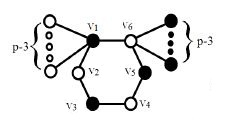
\includegraphics{sample2.jpg}
\end{center}
\caption{A Monocyclic Graph $C_6(p-3,p-3)$}
\label{fig:c6(p-3,p-3)}
\end{figure}

\begin{figure}[ht]
\begin{center}
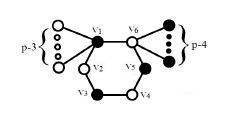
\includegraphics{sample3.jpg}
\end{center}
\caption{A Monocyclic Graph $C_6(p-3,p-4)$}
\label{fig:c6(p-3,p-4)}
\end{figure}

\begin{figure}[!ht]
\begin{center}
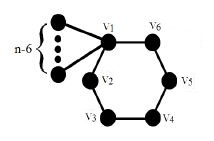
\includegraphics{sample4.jpg}
\end{center}
\caption{A Monocyclic Graph $C_6(n-6,0)$}
\label{fig:c6(n-6,0)}
\end{figure}

\begin{e.g.}\rm
Take $C_6(s,t)$ be a monocyclic graph with $C_6$ as its cycle, we now verify the results in \cite{wiener_ind_bipart} using Theorem \ref{thm:wiener_ckst}:
\begin{enumerate}
\item {$W(C_6(p-3,p-3))=5p^2-2p-12$, where $p\geq 4$.\\
Now, in figure \ref{fig:c6(p-3,p-3)}
$W(C_6(p-3,p-3))=\frac{1}{2}[2(p-3)^2+2(p-3)^2-2(p-3)-2(p-3)+6(p-3)(p-3)+9(2(p-3)+2(p-3)+6)+12(p-3)+12(p-3)]$, then we have $W(C_6(p-3,p-3))=\frac{1}{2}[10(p-3)^2+56(p-3)+54]$. Simply the results, we now have
$$
W(C_6(p-3,p-3))=\frac{1}{2}(10p^2-4p-24)=5p^2-2p-12
$$ 
and we are done.
}

\item {$W(C_6(p-3,p-4))=5p^2-7p-10$, where $p\geq 4$.\\
Now, in figure \ref{fig:c6(p-3,p-4)}
$W(C_6(p-3,p-4))=\frac{1}{2}[2(p-3)^2+2(p-4)^2-2(p-3)-2(p-4)+6(p-3)(p-4)+9(2(p-3)+2(p-4)+6)+12(p-3)+12(p-4)]$, then we have $W(C_6(p-3,p-4))=\frac{1}{2}[2(p-3)^2+2(p-4)^2+6(p-3)(p-4)+28(p-3)+28(p-4)+54]$. Simply the results, we now have
$$
W(C_6(p-3,p-4))=\frac{1}{2}(10p^2-14p-20)=5p^2-7p-10
$$ 
and we are done.}

\item {$W(C_6(n-6,0))=n^2+2n-21$, where $n\geq 6$.\\
Now, in figure \ref{fig:c6(n-6,0)}
$W(C_6(n-6,0))=\frac{1}{2}[2(n-6)^2+2(0)^2-2(n-6)-2(0)+6(n-6)(0)+9(2(n-6)+2(0)+6)+12(n-6)+12(0)]$, then we have $W(C_6(n-6,0))=\frac{1}{2}[2(n-6)^2+28(n-6)+54]$. Simply the results, we now have
$$
W(C_6(n-6,0))=\frac{1}{2}(2n^2-4n-42)=n^2-2n-21
$$ 
and we are done.}
\end{enumerate}
\end{e.g.}


\section{Zagreb Index of Monocyclic Graph $C_k(s,t)$}

\begin{thm}\rm
Suppose we partition the vertex set of monocyclic graph $C_k(s,t)$ into $G_s,G_k$ and $G_t$. Then the \textbf{Zagreb index} of $C_k(s,t)$ is
\begin{equation}
Zg(C_k(s,t))=s^2+t^2+8s+8t+4k
\label{eqn:zagreb}
\end{equation}
\label{thm:zagreb_mg} 
\end{thm}
\proof Given sets $G_s,G_k$, and $G_t$ wherein $V(C_k(s,t))=G_s\cup G_k\cup G_t$, it is evident that $|G_1|=s$, $|G_2|=k$, and $|G_3|=t$. Since, $deg(u)=2,\forall u\in G_s$, $deg(u)=2,\forall u \in G_t, deg(u)=2, \forall u \in G_k-{v_1,v_k} $, where $v_1$ and $v_2$ are the two adjacent vertices where \textbf{pendant vertices} $G_s$ and $G_t$ are attached respectively. Note that, $deg(v_1)=s+2$ and $deg(v_k)=t+2$. By definition \href{chap2.tex}{\ref{sec:m1(g)}} \textbf{Zagreb index} of monocyclic graph $C_k(s,t)$ is $Zg(C_k(s,t))=s(deg(u\in G_s))^2+t(deg(u\in G_t))^2+(s+2)^2+(t+2)^2+(k-2)(deg(u\in G_k-\left\lbrace v_1,v_k \right\rbrace))$. Simplifying further we have, $s(1^2)+t(1^2)+(s+2)^2+(t+2)^2+(k-1)(2^2)$ which is equal to $s^2+t^2+5s+5t+4k$. \medskip 

Thus, \textbf{Zagreb index} of $C_k(s,t)$ is $Zg(C_k(s,t))=s^2+t^2+5s+5t+4k$. \qed

\begin{e.g.}\rm
In figure \ref{fig:c4(2,3)}, the Zagreb index of the graph would be, $1^2+1^2+4^2+2^2+2^2+5^2+1^2+1^2+1^2=54$. Using equation \ref{eqn:zagreb} we have $Zg(C_4(2,3))=2^2+3^2+5(2)+5(3)+4(4)=54$.
\end{e.g.}

\begin{e.g.}\rm
In figure \ref{fig:c5(3,3)}, the Zagreb index of the graph would be, $1^2+1^2+1^2+5^2+2^2+2^2+2^2+5^2+1^2+1^2+1^2=68$. Using equation \ref{eqn:zagreb}, $Zg(C5(3,3))=3^2+3^2+5(3)+5(3)+4(5)=68$
\end{e.g.}

\section{Molecular Topological Index of Monocyclic Graph $C_k(s,t)$}
\begin{thm}\rm
Let $x\in V(C_k)$, then the Molecular Topological Index of monocyclic graph $C_k(s,t)$ is 
\begin{equation}
MTI(C_k(s,t))=4s^2+4t^2+6s+6t+10st+2w(x,C_k)(2s+2t+k)+3sk+3kt+4k 
\label{mti_ckst}
\end{equation}
where
$$
w(x,C_k)=\left\lbrace\begin{array}{cc}
\frac{k^2}{4} & $if k is even \\ 
\frac{(k+1)(k-1)}{4} & $if k is odd
\end{array}
$$
\label{thm:mti_mg}
\end{thm}

\proof
Using definition \href{chap2.tex}{\ref{sec:s_mti}}, we can now safely evaluate the \textbf{MTI} of the monocyclic graph $C_k(s,t)$.

Now that we calculated the degree distance index by Theorem \ref{thm:dd_mg} and the zagreb index using Theorem \ref{thm:zagreb_mg} by simple algebraic manipulation we arrived at Theorem \ref{thm:mti_mg}.
\qed

\begin{e.g.}\rm
In figure \ref{fig:c4(2,3)}, Degree distance index and Zagreb index are solved. Found that $DD(C_4(2,3))=261$ and $Zg(C_k(s,t))=54$. This would yield to an $MTI(C_4(2,3))=261+54=315$. Using Theorem \ref{thm:mti_mg}, $MTI(C_4(2,3))=4(2^2)+4(3^2)+3(2)+3(3)+10(2)(3)+2(4)(2(2)+2(3)+4)+3(2)(4)+3(4)(3)+4(4)=315$.
\end{e.g.}

\begin{e.g.}\rm
In figure \ref{fig:c5(3,3)}, Degree distance index and Zagreb index are already solved. The values are the following, $DD(C_5(3,3))=426$ and $Zg(C_5(3,3))=68$. Hence, $MTI(C_5(3,3))=426+68=494$. Using Theorem \ref{thm:mti_mg}, $MTI(C_5(3,3))=4(3^2)+4(3^2)+3(3)+3(3)+10(3)(3)+2(6)(2(3)+2(3)+5)+3(3)(5)+3(5)(3)+4(5)=494$.
\end{e.g.}

\begin{table}[!ht]
\caption{Degree Distance Index of $C_4(2,3)$ at $x$ by Inspection}
\begin{center}
\begin{tabular}{|c|c|c|c|c|}
\hline 
$x\in V(C_k(s,t))$ & $deg (x)$ & $w(x,C_k(s,t))$ & $dd(v_x,C_k(s,t))$  \\ 
\hline 
$x=v_1$ & 4 & 12 & 48 \\ 
\hline 
$x=v_4$ & 5 & 11 & 55 \\ 
\hline 
$x=v_2$ & 2 & 17 & 34 \\ 
\hline 
$x=v_3$ & 2 & 16 & 32 \\ 
\hline 
$x=u_1$ & 1 & 19 & 19 \\ 
\hline 
$x=u_2$ & 1 & 19 & 19 \\ 
\hline
$x=w_1$ & 1 & 18 & 18 \\ 
\hline 
$x=w_2$ & 1 & 18 & 18 \\ 
\hline 
$x=w_3$ & 1 & 18 & 18 \\ 
\hline 
$TOTAL$ & 18 & 148 & 261 \\ 
\hline 
\end{tabular} 
\end{center}
\label{tab:DD_c4_inspection}
\end{table}

\newpage
\begin{table}[!ht]
\caption{Degree Distance Index of $C_5(3,3)$ at $x$ by Inspection}
\begin{center}
\begin{tabular}{|c|c|c|c|c|}
\hline 
$x\in V(C_k(s,t))$ & $deg (x)$ & $w(x,C_k(s,t))$ & $dd(v_x,C_k(s,t))$  \\ 
\hline 
$x=v_1$ & 5 & 15 & 75 \\ 
\hline 
$x=v_5$ & 5 & 15 & 75 \\ 
\hline 
$x=v_2$ & 2 & 21 & 42 \\ 
\hline 
$x=v_3$ & 2 & 24 & 48 \\ 
\hline 
$x=v_3$ & 2 & 21 & 42 \\ 
\hline 
$x=u_1$ & 1 & 24 & 24 \\ 
\hline 
$x=u_2$ & 1 & 24 & 24 \\ 
\hline 
$x=w_1$ & 1 & 18 & 18 \\ 
\hline
$x=u_3$ & 1 & 24 & 24 \\ 
\hline  
$x=w_2$ & 1 & 18 & 18 \\ 
\hline 
$x=w_1$ & 1 & 24 & 24 \\ 
\hline 
$x=w_2$ & 1 & 24 & 24 \\ 
\hline 
$x=w_3$ & 1 & 24 & 24 \\ 
\hline 
$TOTAL$ & 22 & 240 & 426 \\ 
\hline 
\end{tabular} 
\end{center}
\label{tab:DD_c4_inspection}
\end{table}

\begin{table}[!ht]
\caption{Molecular Topological Index of Some Monocyclic Graph $C_k(s,t)$}
\begin{center}
\begin{tabular}{|c|c|c|c|c|c|}
\hline 
$k-cycles$ & $s$ & $t$ & $DD(C_k(s,t))$ & $Zg(C_k(s,t))$ & $MTI$ \\  
\hline 
$4$ & 2 & 3 & 261 & 69 & 330 \\ 
\hline 
$4$ & 3 & 3 & 332 & 82 & 414 \\ 
\hline 
$4$ & 5 & 5 & 692 & 146 & 838 \\ 
\hline 
$5$ & 2 & 3 & 344 & 73 & 417 \\ 
\hline 
$5$ & 4 & 4 & 612 & 116 & 728 \\ 
\hline 
$5$ & 10 & 10 & 2400 & 380 & 2780 \\ 
\hline
\end{tabular} 
\end{center}
\label{tab:mti_some_mg}
\end{table}




%\chapter{Summary and Recommendation}
\label{chap:summary}

\section{Summary}
Let $C_k(s,t)$ be a monocyclic graph with $s$ and $t$ pendant vertices attached to $C_k$ at vertices $v_1$ and $v_k$ and let $x\in V(C_k)$. In this study, we generalized the formula of the following topological indices:
\begin{enumerate}
\item {Wiener Index of Monocyclic Graph $C_k(s,t)$\\
$$
W(C_k(s,t))=\frac{1}{2}[2s^2+2t^2-2s-2t+6st+w(x,C_k)(2s+2t+k)+2ks+2kt]
}

\item {Degree Distance Index of Monocyclic Graph $C_k(s,t)$\\
$$
DD(C_k(s,t))=3s^2+3t^2-2s-2t+10st+2w(x,C_k)(2s+2t+k)+3ks+3kt
}

\item {Zagreb Index of $C_k(s,t)$\\
$$
Zg(C_k(s,t))=s^2+t^2+8s+8t+4k
$$
}

\item {Molecular Topological Index of $C_k(s,t)$\\
$$
MTI(C_k(s,t))=4s^2+4t^2+6s+6t+10st+2w(x,C_k)(2s+2t+k)+3sk+3kt+4k
$$
}
\end{enumerate}
where $
w(x,C_k)=\left\lbrace\begin{array}{cc}
\frac{k^2}{4} & $if k is even \\ 
\frac{k(k+1)(k-1)}{4} & $if k is odd
\end{array}
$
\\
\section{Recommendation}
Now that we had generalized the topological indices in the previous chapters by using the parameters $k,s,$ and $t$, we can also calculate other topological indices for future studies. On the other hand, instead of using Monocyclic Graphs we can also pick other graphs like the Sunflower Graph, Spiderweb or Cobweb Graph and others.

\medskip In this study, we assume $v_1$ and $v_k$ to be adjacent. What if $v_1$ and $v_k$ are not adjacent? Perhaps, we could start another study in relation to this as an extension of this paper. We could also study a specific monocyclic graph with all vertices at $C_k$ attached with pendant vertices.    


\appendix
%\input{newfile}
\nocite*

\bibliographystyle{siam}
\bibliography{bibliog}
%to edit your bibliography, open the BIBLIOG.BIB file.

\end{document}

